\documentclass[10pt,a4paper]{article}
\usepackage[latin1]{inputenc}
\usepackage{amsmath}
\usepackage{amsfonts}
\usepackage{amssymb}
\usepackage{graphicx}
\usepackage{float}
\begin{document}
\section{Semantic Tableaux for first-order logic}

\begin{center}
\textbf{Quantifier rules for Semantic Tableaux}
\end{center}
\begin{tabular}{l c l c}
($ \forall $ T) &  \parbox{5cm}{\centering$ \forall x A(x) : $ T
\newline
$ \downarrow $
\newline
$ A(t/x) : $ T
\newline
for any term \textit{t} occurring on this branch and free for \textit{x} in \textit{A}} & ($ \exists $ T)* & \parbox{5cm}{\centering$ \exists x A(x) : $ T
\newline
$ \downarrow $
\newline
$ A(c/x) : $ T
\newline
for a \textit{new} constant symbol \textit{c} not yet occurring on this branch}  \\[1.5cm]

($ \exists $ F) & \parbox{5cm}{\centering$ \exists x A(x) : $ F
\newline
$ \downarrow $
\newline
$ A(t/x) : $ F
\newline
for any term \textit{t} occurring on this branch and free for \textit{x} in \textit{A}} & ($ \forall $ F)*  & \parbox{5cm}{\centering$ \forall x A(x) : $ F
\newline
$ \downarrow $
\newline
$ A(c/x) : $ F
\newline
for a \textit{new} constant symbol \textit{c} not yet occurring on this branch}  \\
\end{tabular}

(*) \textit{This rule may only be applied once for the given formula on each branch}

Here are some examples of a semantic tableaux with first-order logic \cite[p. 46]{LecPartII}.

\begin{figure}[H]
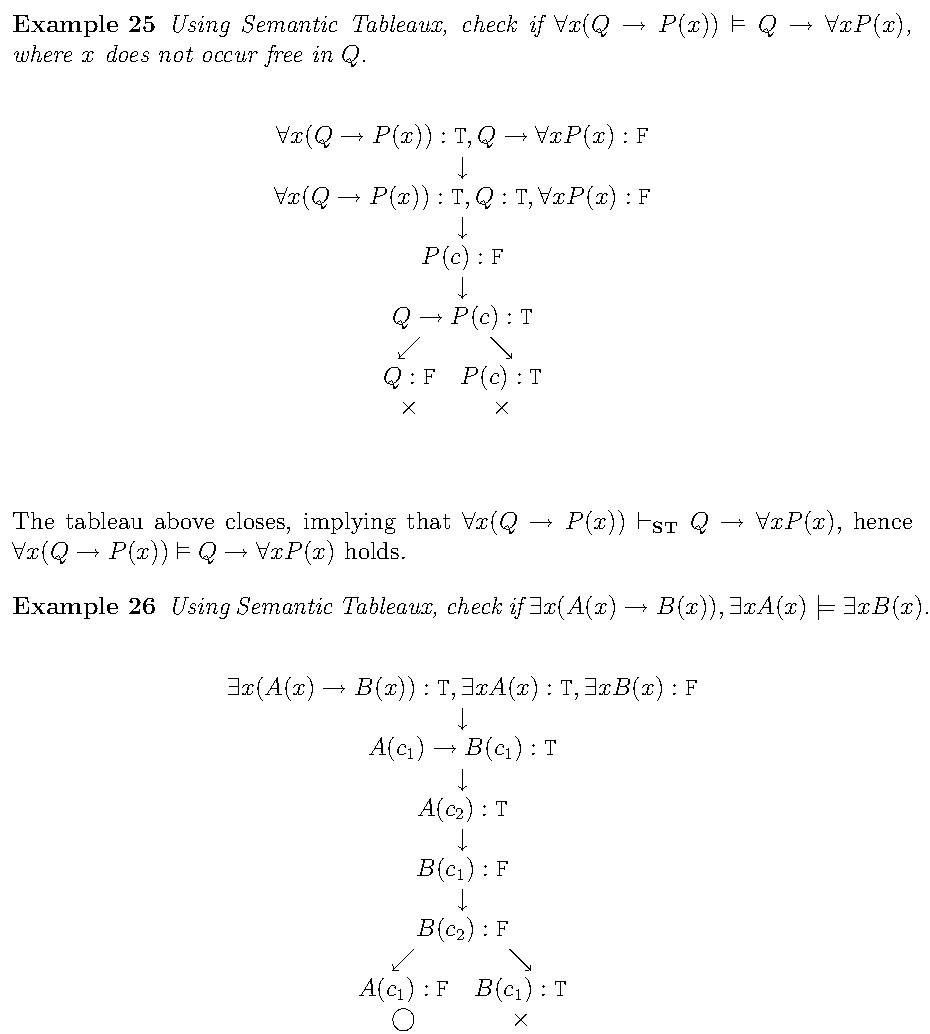
\includegraphics[scale=0.6]{./figures/tableaux.pdf}
\end{figure}

\section{Prenex and clausal normal forms}
\subsection{Negating first-order formulae. Negation normal form}

\textit{Negation normal form}\cite[p.58]{LecPartII} means that negations only occurs in front of atomic formulae. eg:

\begin{figure}[H]
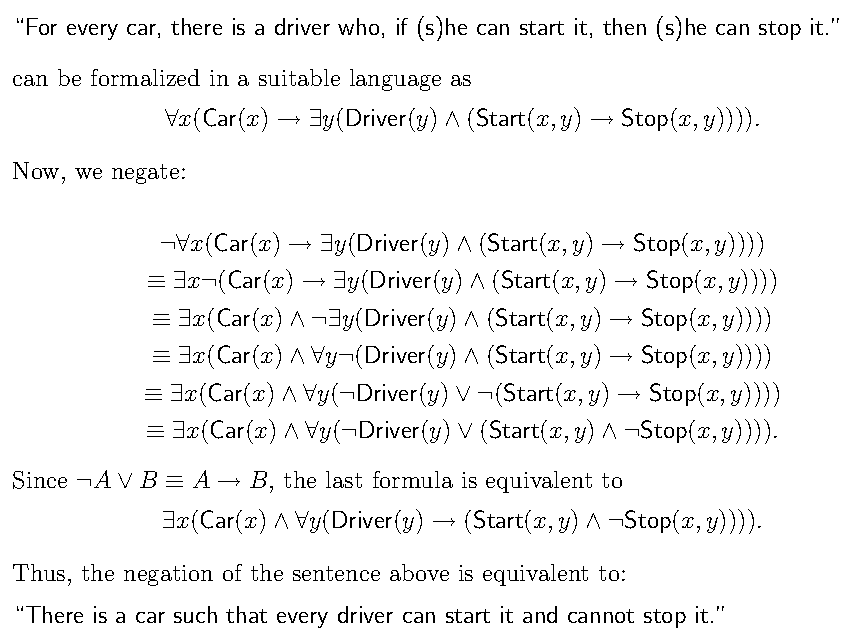
\includegraphics[scale=0.6]{./figures/negnormform.pdf}
\end{figure}

\subsection{Prenex normal forms}

\textit{Prenex normal forms} \cite[p. 59]{LecPartII} refer to a form of the formula where all the quantifications have been moved to the outermost scope like:
$$ Q_1 x_1 .. Q_n x_n A $$

where $ Q_n $ is all the quantifiers called the \textbf{prefix} and $ A $ is the formula called the \textbf{matrix}

If the formula itself is in either CNF or DNF then we refer to the formula as a \textit{prenex CNF / PCNF} or \textit{prenex DNF / PDNF}

\textbf{Algorithm for construction these normal forms:}

\begin{enumerate}
\item Eliminate all occurences of $ \to $ and $ \leftrightarrow $ as in the propositional case.
\item Import all negations inside all other logical connectives and transform the formula to negation normal form.
\item Pull all quantifiers in front and thus transform the formula into a prenex form.

For that use the equivalences:
      \begin{enumerate}
\item $ \forall x P \land \forall x Q \equiv \forall x(P \land Q) $
\item $ \exists x P \lor \exists x Q \equiv \exists(P \lor Q) $

to pull some quantifiers outwards and, after renaming the formula \textit{wherever necessary}.

Then, use also the following equivalences, where \textit{x} does not occur free in \textit{Q}, until the formula is transformed to a prenex form:

\item $ \forall x P \land Q \equiv Q \land \forall x P \equiv \forall x(P\land Q) $
\item $ \forall x P \lor Q \equiv Q \lor \forall x P \equiv \forall x(P \lor Q) $
\item $ \exists x P \lor Q \equiv Q \lor \exists x P \equiv \exists x (P \lor Q) $
\item $ \exists x P \land Q \equiv Q \land \exists x P \equiv \exists x(P\land Q) $
\end{enumerate}
\item Finally, transform the matrix in a DNF or CNF, just like a propositional formula.
\end{enumerate}

Here are some examples:
\begin{figure}[H]
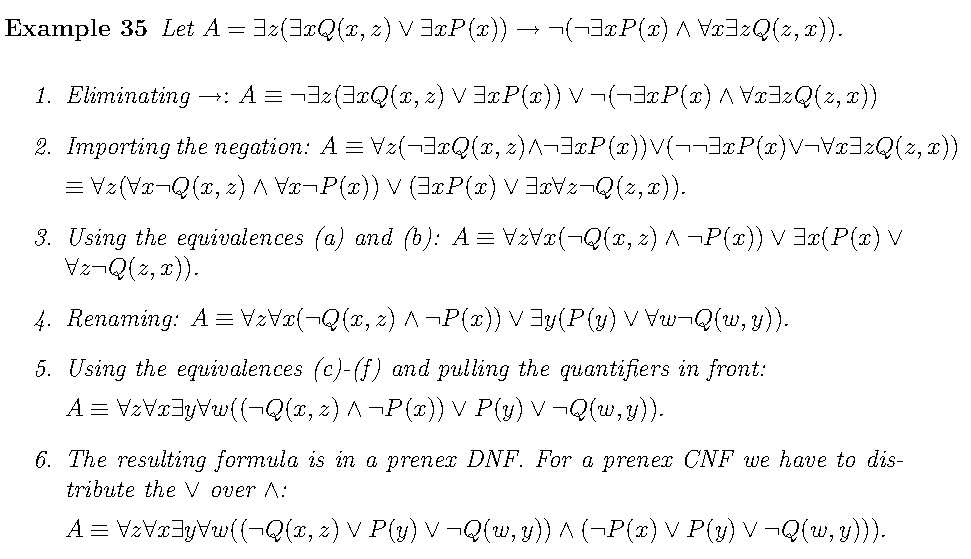
\includegraphics[scale=0.6]{./figures/prenexex.pdf}
\end{figure}

\subsection{Skolemization}

Skolemization\cite[p. 60]{LecPartII} is a procedure used to eliminate the existential quantifiers in a first-order formula in a prenex form by a uniform replacement of all occurrences of existentially
quantified individual variables with terms headed by new functional symbols, called
\textit{Skolem functions}.\\

\textit{Skolem functions} take as arguments all variables (if any) which are bound by universal quantifiers in the scope of which the given existential quantifier sits. In particular, existentially quan-
tified variables not in the scope of any universal quantifiers are replaced by constant symbols, called \textit{Skolem constants}.

\textbf{Examples of skolemization}
\begin{figure}[H]
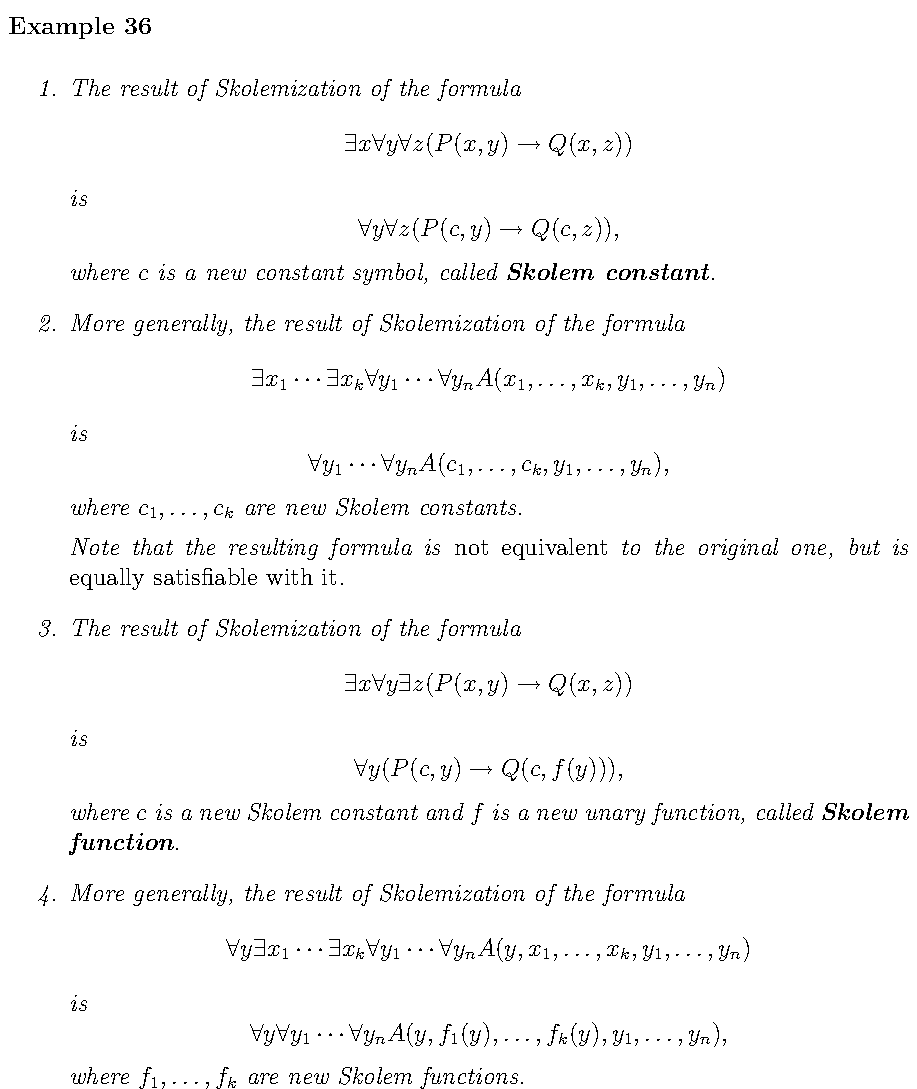
\includegraphics[scale=0.6]{./figures/skolemex1.pdf}
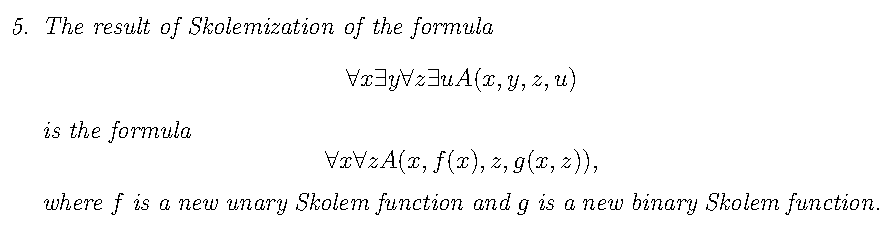
\includegraphics[scale=0.6]{./figures/skolemex2.pdf}
\end{figure}


\subsection{Clausal form}

\textit{Clausal forms} \cite[p. 62]{LecPartII} is a set of \textit{literals} (representing their disjunction).

All clauses are implicitly assumed to be universally quantified.

\textbf{The algorithm for transforming any formula into clausal form}

\begin{itemize}
\item Transform \textit{A} into prenex CNF
\item Skolemize all existential quantifiers.
\item Remove all universalt quantifiers.
\item Wrute the \textit{matrix} (which is in CNF) as a set of clauses.
\end{itemize}

\begin{figure}[H]
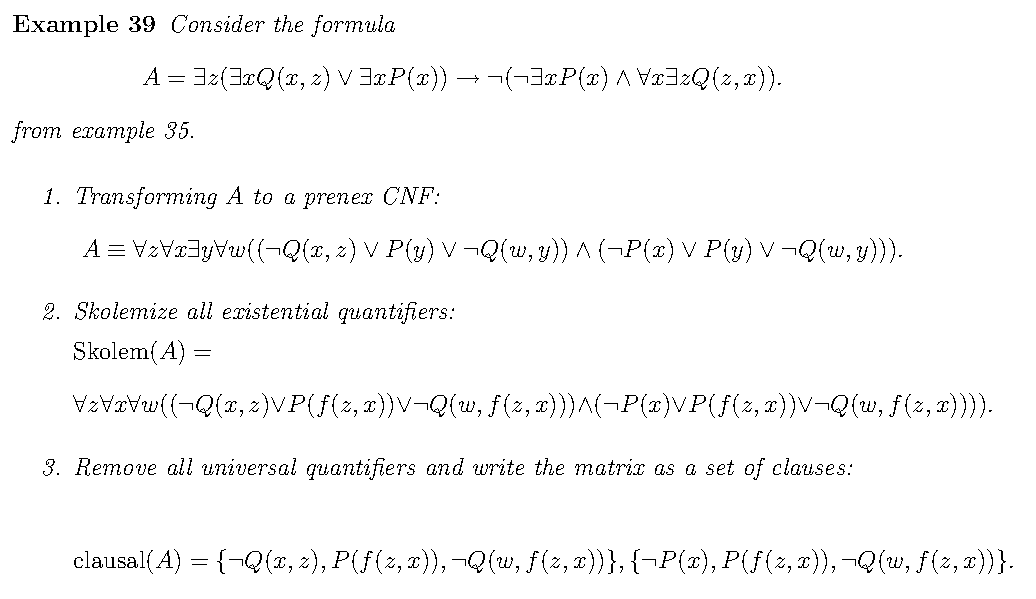
\includegraphics[scale=0.6]{./figures/clausalex.pdf}
\end{figure}

\end{document} 